\documentclass{standalone}
\usepackage{tikz}
\usetikzlibrary{calc}
\begin{document}
    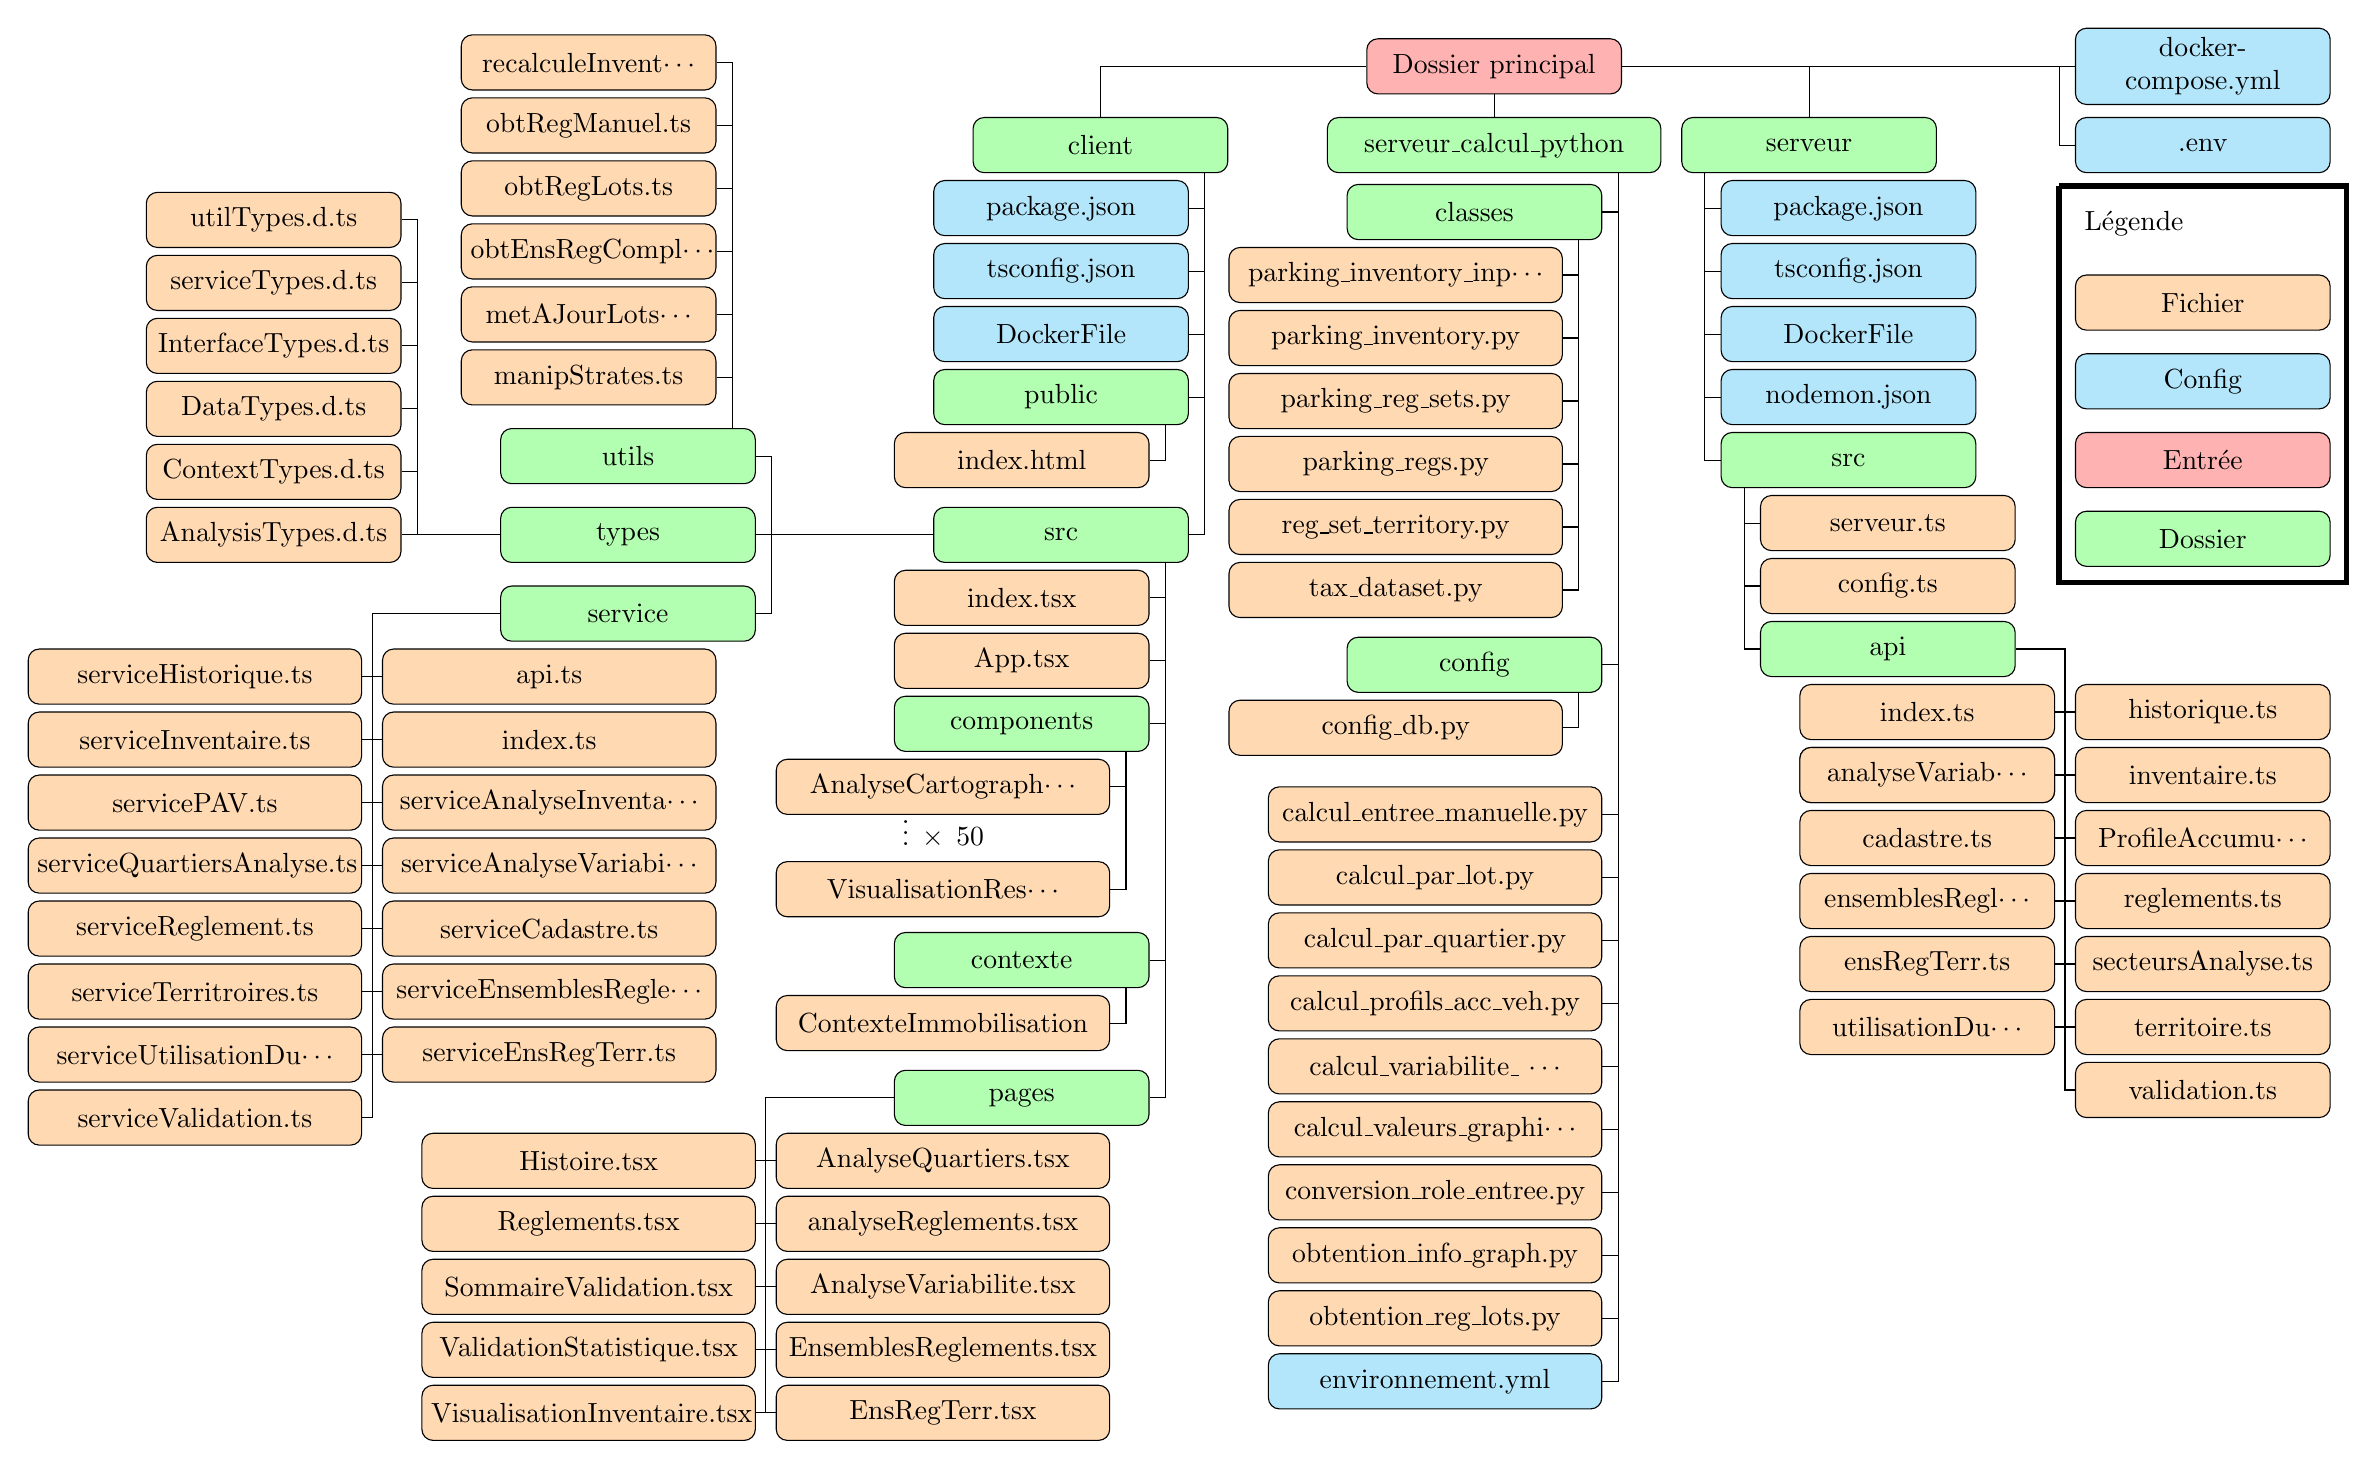
\begin{tikzpicture}
        \tikzstyle {dossier} = [rectangle, rounded corners, text width=3cm, minimum height=0.7cm,text centered,  draw=black, fill=green!30]
        \tikzstyle {fichier} = [rectangle, rounded corners, text width=3cm, minimum height=0.7cm,text centered,  draw=black, fill=orange!30]
        \tikzstyle {fichierconfig} = [rectangle, rounded corners, text width=3cm, minimum height=0.7cm,text centered,  draw=black, fill=cyan!30]
        \tikzstyle {dossierparent} = [rectangle, rounded corners, text width=3cm, minimum height=0.7cm,text centered,  draw=black, fill=red!30]
        % Top levle
        \node(doss_princ) [dossierparent]{Dossier principal};
            \node(dock-comp)[fichierconfig,right of=doss_princ,xshift=8cm]{docker-compose.yml};
            \node(dotenv)[fichierconfig,below of=dock-comp,yshift=0.0cm]{.env};
        % serveur calcul python
        \node(serveur-python)[dossier,below of=doss_princ,text width = 4cm]{serveur\_calcul\_python};
            \node(classes-python) [dossier,below of=serveur-python,xshift=-0.25cm,yshift=0.15cm]{classes};
                \node(pii) [fichier,below of=classes-python,xshift=-1cm,text width=4cm,yshift=0.2cm]{parking\_inventory\_inp$\cdots$};
                \node(pi)[fichier,below of=pii,text width=4cm,yshift=0.2cm]{parking\_inventory.py};
                \node(prs)[fichier,below of=pi,text width =4cm,yshift=0.2cm]{parking\_reg\_sets.py};
                \node(pr)[fichier,below of=prs,text width = 4cm,yshift=0.2cm]{parking\_regs.py};
                \node(rst)[fichier, below of=pr,text width = 4cm,yshift=0.2cm]{reg\_set\_territory.py};
                \node(td)[fichier,below of=rst,text width = 4cm,yshift=0.2cm]{tax\_dataset.py};
                \coordinate(target-classes-py) at ($(pii.east|-classes-python.south)+(0.2,0)$);
                \draw (pii.east)-|(target-classes-py);
                \draw (pi.east) -| ($(pii.east-|target-classes-py)$);
                \draw (prs.east) -| ($(pi.east-|target-classes-py)$);
                \draw (pr.east) -| ($(prs.east-|target-classes-py)$);
                \draw (rst.east) -| ($(pr.east-|target-classes-py)$);
                \draw (td.east) -| ($(rst.east-|target-classes-py)$);
            \node(config-python) [dossier,below of=classes-python,yshift=-4.75cm]{config};
                \node(cf_db) [fichier,below of=config-python,xshift=-1cm,text width=4cm,yshift=0.2cm]{config\_db.py};
                \draw(cf_db) -| ($(config-python.south-|cf_db.east)+(0.2,0)$);
            \node(calcul-ent-man) [fichier, below of=serveur-python,yshift=-7.5cm,text width=4cm,xshift=-0.75cm]{calcul\_entree\_manuelle.py};
            \node(calcul-par-lot)[fichier,below of=calcul-ent-man,text width=4cm,yshift=0.2cm]{calcul\_par\_lot.py};
            \node(calcul-par-quartier)[fichier,below of=calcul-par-lot,text width=4cm,yshift=0.2cm]{calcul\_par\_quartier.py};
            \node(calcul-pav)[fichier,below of=calcul-par-quartier,text width=4cm,yshift=0.2cm]{calcul\_profils\_acc\_veh.py};
            \node(calcul-var)[fichier,below of=calcul-pav,text width=4cm,yshift=0.2cm]{calcul\_variabilite\_ $\cdots$};
            \node(calcul-val-graph)[fichier,below of=calcul-var,text width=4cm,yshift=0.2cm]{calcul\_valeurs\_graphi$\cdots$};
            \node(convers-role-rentree)[fichier,below of=calcul-val-graph,text width=4cm,yshift=0.2cm]{conversion\_role\_entree.py};
            \node(obtention-info-graph)[fichier,below of=convers-role-rentree,text width=4cm,yshift=0.2cm]{obtention\_info\_graph.py};
            \node(obtention-reg-lots)[fichier,below of=obtention-info-graph,text width=4cm,yshift=0.2cm]{obtention\_reg\_lots.py};
            \node(environyml)[fichierconfig,below of=obtention-reg-lots,yshift=0.2cm,text width=4cm]{environnement.yml};
            \coordinate(target-serveur-py) at ($(classes-python.east|-serveur-python.south)+(0.2,0)$);
            \draw(classes-python.east)-|(target-serveur-py);
            \draw(config-python.east) -|($(classes-python.east-|target-serveur-py)$);
            \draw(calcul-ent-man.east) -|($(config-python.east-|target-serveur-py)$);
            \draw(calcul-par-lot.east) -|($(calcul-ent-man.east-|target-serveur-py)$);
            \draw(calcul-par-quartier.east) -|($(calcul-par-lot.east-|target-serveur-py)$);
            \draw(calcul-pav.east) -|($(calcul-par-quartier.east-|target-serveur-py)$);
            \draw(calcul-var.east) -|($(calcul-pav.east-|target-serveur-py)$);
            \draw(calcul-val-graph.east) -|($(calcul-var.east-|target-serveur-py)$);
            \draw(convers-role-rentree.east) -|($(calcul-val-graph.east-|target-serveur-py)$);
            \draw(obtention-info-graph.east) -|($(convers-role-rentree.east-|target-serveur-py)$);
            \draw(obtention-reg-lots.east) -|($(obtention-info-graph.east-|target-serveur-py)$);
            \draw(environyml.east) -|($(obtention-reg-lots.east-|target-serveur-py)$);
        % Serveur
        \node(serveur) [dossier,right of=serveur-python,xshift=3cm]{serveur};
            \node(packge-serv)[fichierconfig,below of=serveur,xshift=0.5cm,yshift=0.2cm]{package.json};
            \node(tsconfig-serv)[fichierconfig,below of=packge-serv,yshift=0.2cm]{tsconfig.json};
            \node(dckerfile-serv)[fichierconfig,below of=tsconfig-serv,yshift=0.2cm]{DockerFile};
            \node(nodemon-serv)[fichierconfig,below of=dckerfile-serv,yshift=0.2cm]{nodemon.json};
            \node(src-serv)[dossier,below of=nodemon-serv,yshift=0.2cm]{src};
                \node (serveur-ent)[fichier,below of=src-serv,xshift=0.5cm,yshift=0.2cm]{serveur.ts};
                \node (serveur-cfg)[fichier,below of=serveur-ent,yshift=0.2cm]{config.ts};
                \node (api-serv)[dossier,below of=serveur-cfg,yshift=0.2cm]{api};
                    \node (index-serv-api)[fichier,below of=api-serv,xshift=0.5cm,yshift=0.2cm]{index.ts};
                    \node (ana-quart-serv)[fichier,below of=index-serv-api,yshift=0.2cm]{analyseQuartier.ts};
                    \node (ana-var-serv)[fichier,below of=index-serv-api,yshift=0.2cm]{analyseVariab$\cdots$};
                    \node (cad-serv)[fichier,below of=ana-var-serv,yshift=0.2cm]{cadastre.ts};
                    \node (ens-reg-serv) [fichier,below of=cad-serv,yshift=0.2cm]{ensemblesRegl$\cdots$};
                    \node (ens-reg-terr-serv) [fichier,below of=ens-reg-serv,yshift=0.2cm]{ensRegTerr.ts};
                    \node (util-sol-serv)[fichier,below of=ens-reg-terr-serv,yshift=0.2cm]{utilisationDu$\cdots$};
                    \node (histo-serv) [fichier,right of=index-serv-api,xshift=2.5cm]{historique.ts};
                    \node (inventaire-serv) [fichier,below of=histo-serv,yshift=0.2cm]{inventaire.ts};
                    \node (PAV-serv)[fichier,below of=inventaire-serv,yshift=0.2cm]{ProfileAccumu$\cdots$};
                    \node (reg-serv)[fichier,below of=PAV-serv,yshift=0.2cm]{reglements.ts};
                    \node (sect-serv) [fichier,below of=reg-serv,yshift=0.2cm]{secteursAnalyse.ts};
                    \node (terr-serv) [fichier,below of=sect-serv,yshift=0.2cm]{territoire.ts};
                    \node (valid-serv)[fichier,below of=terr-serv,yshift=0.2cm]{validation.ts};
                    \coordinate(src-serv-targ) at ($(index-serv-api.east)!0.5!(histo-serv.west)$);
                    \draw (index-serv-api.east)--(histo-serv.west);
                    \draw (api-serv.east)-|(src-serv-targ);
                    \draw (valid-serv.west)-|(src-serv-targ);
                    \draw (ana-var-serv.east) -- (inventaire-serv.west);
                    \draw (cad-serv.east) --(PAV-serv.west);
                    \draw (ens-reg-serv.east) -- (reg-serv.west);
                    \draw (ens-reg-terr-serv.east) --(sect-serv.west);
                    \draw (util-sol-serv.east) -- (terr-serv.west);
                \coordinate (src-serv-target) at ($(src-serv.south-|serveur-ent.west)+(-0.2,0)$);
                \draw (serveur-ent.west) -| (src-serv-target) ;
                \draw (serveur-cfg.west) -| ($(serveur-ent.west-|src-serv-target)$);
                \draw (api-serv.west) -| ($(serveur-cfg.west-|src-serv-target)$);
            \coordinate(target-serveur-bot) at ($(serveur.south-|packge-serv.west)+(-0.2,0)$);
            \draw (target-serveur-bot) |-(packge-serv.west);
            \draw (tsconfig-serv.west) -|($(packge-serv.west-|target-serveur-bot)$);
            \draw (dckerfile-serv.west) -|($(tsconfig-serv.west-|target-serveur-bot)$);
            \draw (nodemon-serv.west) -|($(dckerfile-serv.west-|target-serveur-bot)$);
            \draw (src-serv.west) -|($(nodemon-serv.west-|target-serveur-bot)$);
        % Client
        \node(client)[dossier, left of=serveur-python,xshift=-4cm]{client};
            \node(package-clt)[fichierconfig,below of=client,xshift=-0.5cm,yshift=0.2cm]{package.json};
            \node(tsconfig-clt)[fichierconfig,below of=package-clt,yshift=0.2cm]{tsconfig.json};
            \node(dockerfile-clt)[fichierconfig,below of=tsconfig-clt,yshift=0.2cm]{DockerFile};
            \node(public) [dossier,below of=dockerfile-clt,yshift=0.2cm]{public};
                \node(indexh) [fichier,below of=public,xshift=-0.5cm,yshift=0.2cm]{index.html};
                \draw (indexh.east) -| ($(indexh.east|-public.south)+(0.2,0)$);
            \node(src-clt)[dossier,below of=public,yshift=-.75cm]{src}; 
                \node(indext)[fichier,below of=src-clt,xshift=-0.5cm,yshift=0.2cm]{index.tsx};
                \coordinate (target-first-src) at ($(indext.east|-src-clt.south)+(0.2,0)$);
                
                \node(appt)[fichier,below of=indext,yshift=0.2cm]{App.tsx};
                \node(comps-clt)[dossier,below of=appt,yshift=0.2cm]{components};
                    \node(ana-carto-quartiers)[fichier,below of=comps-clt,xshift=-1cm,text width =4cm,yshift=0.2cm]{AnalyseCartograph$\cdots$};
                    \node(dots)[below of=ana-carto-quartiers, text width =4cm,text centered,yshift=0.5cm]{$\vdots \times 50$};
                    \node(vis-reg-ana-var-fonc)[fichier,below of=dots,text width=4cm,yshift=0.2cm]{VisualisationRes$\cdots$};
                    \coordinate (target-comps) at ($(comps-clt.south-|ana-carto-quartiers.east)+(0.2,0)$);
                    \draw (ana-carto-quartiers.east)-|(target-comps);
                    \draw (vis-reg-ana-var-fonc.east)-|($(comps-clt.south-|target-comps)$);
                \node(context-clt)[dossier,below of=comps-clt,yshift=-2cm]{contexte};
                    \node(contexte)[fichier,below of=context-clt,xshift=-1cm,text width=4cm,yshift=0.2cm]{ContexteImmobilisation};
                    \draw (contexte.east) -|($(contexte.east|-context-clt.south)+(0.2,0)$);
                \node(pages-clt)[dossier,below of=context-clt,yshift=-0.75cm]{pages};
                    \node(ana-quart)[fichier,below of=pages-clt,xshift=-1cm,text width=4cm,yshift=0.2cm]{AnalyseQuartiers.tsx};
                    \node(ana-reg)[fichier,below of=ana-quart,text width=4cm,yshift=0.2cm]{analyseReglements.tsx};
                    \node(ana-var)[fichier,below of=ana-reg,text width=4cm,yshift=0.2cm]{AnalyseVariabilite.tsx};
                    \node(ens-reg)[fichier,below of=ana-var,text width=4cm,yshift=0.2cm]{EnsemblesReglements.tsx};
                    \node(ens-reg-terr)[fichier,below of=ens-reg,text width=4cm,yshift=0.2cm]{EnsRegTerr.tsx};
                    \node(hist)[fichier,left of=ana-quart,text width=4cm,xshift=-3.5cm]{Histoire.tsx};
                    \node(reg)[fichier,below of=hist,text width=4cm,yshift=0.2cm]{Reglements.tsx};
                    \node(somm-val)[fichier,below of=reg,text width=4cm,yshift=0.2cm]{SommaireValidation.tsx};
                    \node(val)[fichier,below of=somm-val,text width=4cm,yshift=0.2cm]{ValidationStatistique.tsx};
                    \node(vis-inv)[fichier,below of=val,text width=4cm,yshift=0.2cm]{VisualisationInventaire.tsx};
                    \coordinate(target-pages) at ($(hist.east)!0.5!(ana-quart.west)$);
                    \coordinate(target-pages-bot) at ($(vis-inv.east)!0.5!(ens-reg-terr.west)$);
                    \draw (pages-clt.west) -| (target-pages);
                    \draw (hist.east) -- (ana-quart.west);
                    \draw (vis-inv.east) -- (ens-reg-terr.west);
                    \draw (reg.east) --(ana-reg.west);
                    \draw (somm-val.east) -- (ana-var.west);
                    \draw (val.east) -- (ens-reg.west);
                    \draw (target-pages-bot)--(target-pages);
                \node(types-clt)[dossier,left of=src-clt,xshift=-4.5cm]{types};
                    \node(anatypes)[fichier,left of=types-clt,xshift=-3.5cm]{AnalysisTypes.d.ts};
                    \node(contTypes)[fichier,above of=anatypes,yshift=-0.2cm]{ContextTypes.d.ts};
                    \node(DataTypes)[fichier,above of=contTypes,yshift=-0.2cm]{DataTypes.d.ts};
                    \node(intTypes)[fichier,above of=DataTypes,yshift=-0.2cm]{InterfaceTypes.d.ts};
                    \node(serviceTypes)[fichier,above of=intTypes,yshift=-0.2cm]{serviceTypes.d.ts};
                    \node(utilTypes)[fichier,above of=serviceTypes,yshift=-0.2cm]{utilTypes.d.ts};
                    \draw (types-clt.west) -- (anatypes.east);
                    \coordinate (target-types-clt) at ($(anatypes.east) +(0.2,0)$);
                    \draw (contTypes.east) -|(target-types-clt);
                    \draw (DataTypes.east) -| ($(contTypes.east-|target-types-clt)$);
                    \draw (intTypes.east) -| ($(DataTypes.east-|target-types-clt)$);
                    \draw (serviceTypes.east) -| ($(intTypes.east-|target-types-clt)$);
                    \draw (utilTypes.east) -| ($(serviceTypes.east-|target-types-clt)$);
                \node(service-clt)[dossier,below of=types-clt]{service};
                    \node(api-clt)[fichier,below of=service-clt,xshift=-1cm,text width=4cm,yshift=0.2cm]{api.ts};
                    \node(indexservic)[fichier,below of=api-clt,text width=4cm,yshift=0.2cm]{index.ts};
                    \node(servAnaInv)[fichier,below of=indexservic,text width=4cm,yshift=0.2cm]{serviceAnalyseInventa$\cdots$};
                    \node(serviceAnaVar)[fichier,below of=servAnaInv,text width=4cm,yshift=0.2cm]{serviceAnalyseVariabi$\cdots$};
                    \node(serviceCadastre)[fichier,below of=serviceAnaVar,text width=4cm,yshift=0.2cm]{serviceCadastre.ts};
                    \node(serviceER)[fichier,below of=serviceCadastre,text width=4cm,yshift=0.2cm]{serviceEnsemblesRegle$\cdots$};
                    \node(serviceRST)[fichier,below of=serviceER,text width=4cm,yshift=0.2cm]{serviceEnsRegTerr.ts};
                    \node(serviceHist)[fichier,left of=api-clt,text width=4cm,xshift=-3.5cm]{serviceHistorique.ts};
                    \node(serviceInv)[fichier,below of=serviceHist,text width=4cm,yshift=0.2cm]{serviceInventaire.ts};
                    \node(servicePAV)[fichier,below of=serviceInv,text width=4cm,yshift=0.2cm]{servicePAV.ts};
                    \node(servicesQuart)[fichier,below of=servicePAV,text width=4cm,yshift=0.2cm]{serviceQuartiersAnalyse.ts};
                    \node(serviceReglements)[fichier,below of=servicesQuart,text width=4cm,yshift=0.2cm]{serviceReglement.ts};
                    \node(serviceTerr)[fichier,below of=serviceReglements,text width=4cm,yshift=0.2cm]{serviceTerritroires.ts};
                    \node(serviceCUBF)[fichier,below of=serviceTerr,text width=4cm,yshift=0.2cm]{serviceUtilisationDu$\cdots$};
                    \node(serviceVal)[fichier,below of=serviceCUBF,text width=4cm,yshift=0.2cm]{serviceValidation.ts};
                    \coordinate (mid-servs) at ($(serviceHist.east)!0.5!(api-clt.west)$);
                    \draw (service-clt.west) -| (mid-servs);
                    \draw (api-clt.west)--(serviceHist.east);
                    \draw (indexservic.west)--(serviceInv.east);
                    \draw (servicePAV.east) --(servAnaInv.west);
                    \draw (servicesQuart.east) --(serviceAnaVar.west);
                    \draw (serviceReglements.east) -- (serviceCadastre.west);
                    \draw (serviceTerr.east) -- (serviceER.west);
                    \draw (serviceCUBF.east) -- (serviceRST.west);
                    \draw(serviceVal.east) -| (mid-servs);
                \node(utils)[dossier,above of=types-clt]{utils};
                    \node(manipStrates)[fichier,above of=utils,xshift=-.5cm]{manipStrates.ts};
                    \node(majLotInv)[fichier,above of=manipStrates,yshift=-0.2cm]{metAJourLots$\cdots$};
                    \node(obtEnsReg)[fichier,above of=majLotInv,yshift=-0.2cm]{obtEnsRegCompl$\cdots$};
                    \node(obtRegLots)[fichier,above of=obtEnsReg,yshift=-0.2cm]{obtRegLots.ts};
                    \node(obtRegManuel)[fichier,above of=obtRegLots,yshift=-0.2cm]{obtRegManuel.ts};
                    \node(recalculeInventaireLot)[fichier,above of=obtRegManuel,yshift=-0.2cm]{recalculeInvent$\cdots$};
                    \coordinate(utils-clt-target) at ($(utils.north-|manipStrates.east)+(0.2,0)$);
                    \draw (manipStrates.east) -|(utils-clt-target);
                    \draw (majLotInv.east) -|($(manipStrates.east-|utils-clt-target)$);
                    \draw (obtEnsReg.east) -|($(majLotInv.east-|utils-clt-target)$);
                    \draw (obtRegLots.east) -|($(obtEnsReg.east-|utils-clt-target)$);
                    \draw (obtRegManuel.east) -|($(obtRegLots.east-|utils-clt-target)$);
                    \draw (recalculeInventaireLot.east) -|($(obtRegManuel.east-|utils-clt-target)$);
                \draw (indext.east) -| (target-first-src);
                \draw (appt.east)-|($(indext.east-|target-first-src)$);
                \draw (comps-clt.east)-|($(appt.east-|target-first-src)$);
                \draw (context-clt.east)-|($(comps-clt.east-|target-first-src)$);
                \draw (pages-clt.east)-|($(context-clt.east-|target-first-src)$);
                \draw (src-clt.west) -- (types-clt.east);
                \draw (service-clt.east) -| ($(types-clt.east)+(0.2,0)$);
                \draw (utils.east) -| ($(types-clt.east)+(0.2,0)$); 
            \coordinate (client-target) at ($(package-clt.east|-client.south)+(0.2,0)$);
            \draw (package-clt.east) -| (client-target);
            \draw (tsconfig-clt.east) -|($(package-clt.east-|client-target)$);
            \draw (dockerfile-clt.east) -|($(tsconfig-clt.east-|client-target)$);
            \draw (public.east) -|($(dockerfile-clt.east-|client-target)$);
            \draw (src-clt.east) -|($(public.east-|client-target)$);
        \draw(client.north) |-(doss_princ.west);
        \draw(serveur-python.north) --(doss_princ.south);
        \coordinate(target-serveur-princ) at ($(doss_princ.east-|serveur.north)$);
        \draw (serveur.north) --(target-serveur-princ);
        \draw(doss_princ.east)--(dock-comp.west);
        \draw (dotenv)-| ($(dock-comp.west)+(-0.2,0)$);
        % Légende
        \node (legend) [right of=doss_princ,text width=3cm,xshift=8cm,yshift=-2cm]{Légende};
        \coordinate (boite_top_left)at($(legend.north west)+ (-0.2,0.2)$);
        \node (fichier_desc)[fichier,below of=legend]{Fichier};
        \node (fichier_conf)[fichierconfig,below of=fichier_desc]{Config};
        \node (dossier_par)[dossierparent,below of=fichier_conf]{Entrée};
        \node (objet_desc)[dossier,below of=dossier_par]{Dossier};
        \coordinate (boite_bot_rght) at ($(objet_desc.south east)+ (0.2,-0.2)$);
        \draw[line width=2pt] (boite_top_left) -| (boite_bot_rght) -| (boite_top_left);
    \end{tikzpicture}
\end{document}